\documentclass[11pt, oneside]{article} 
\usepackage{geometry}
\geometry{letterpaper} 
\usepackage{graphicx}
	
\usepackage{amssymb}
\usepackage{amsmath}
\usepackage{parskip}
\usepackage{color}
\usepackage{hyperref}

\graphicspath{{/Users/telliott/Github/figures/}}
% \begin{center} \includegraphics [scale=0.4] {gauss3.png} \end{center}

\title{Special points}
\date{}

\begin{document}
\maketitle
\Large

%[my-super-duper-separator]
Special points in triangles include the:

$\bullet$ \  orthocenter:  where altitudes cross

$\bullet$ \  centroid:  where the medians (lines to the midpoints of sides) cross
\begin{center} 
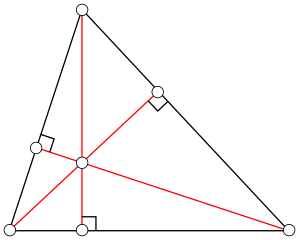
\includegraphics [scale=0.5] {orthocenter.png}
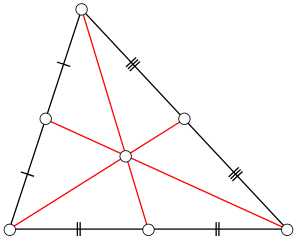
\includegraphics [scale=0.5] {centroid.png} 
\end{center}

$\bullet$ \  circumcenter:  the center of the circle where all three vertices lie, also, where perpendiculars to side midpoints cross

$\bullet$ \  incenter:  where angle bisectors cross
\begin{center} 
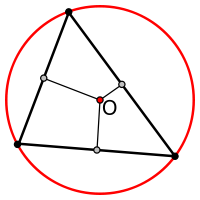
\includegraphics [scale=0.5] {circumcenter.png}
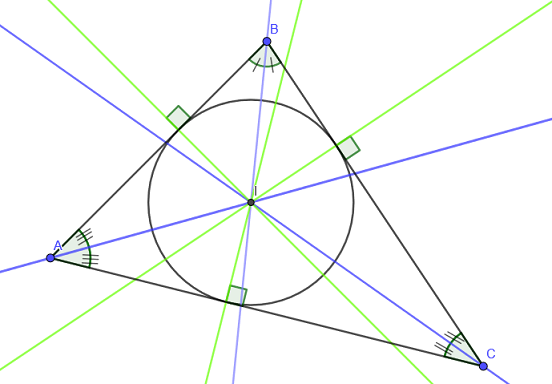
\includegraphics [scale=0.5] {incenter.png} \end{center}

Euler showed that the first three of these points lie on one line.
\begin{center} 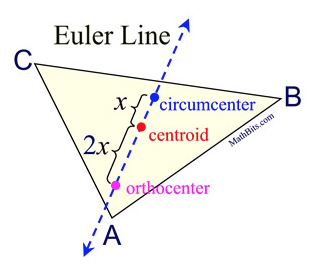
\includegraphics [scale=0.6] {euler_line.png} \end{center}

\subsection*{centroid}
We'll start with the centroid.  The centroid is where bisectors of opposing sides cross.

Consider the triangle in the figure below (left panel).  

\begin{center} 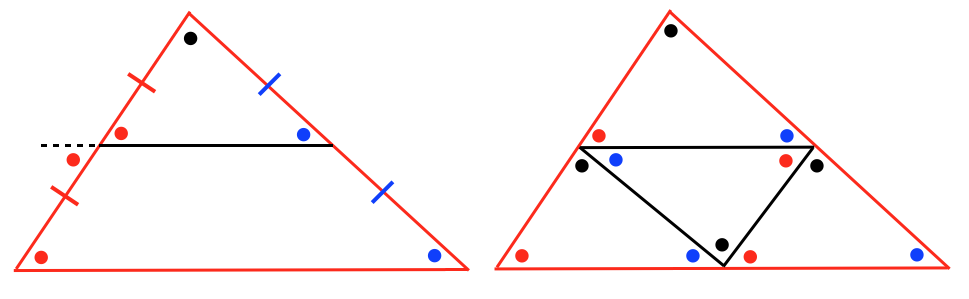
\includegraphics [scale=0.4] {midpoints1.png} \end{center}

Draw a line segment parallel to the base and connecting to the midpoint of the left side.  Then, by the alternate interior angle theorem and the vertical angle theorem, the two angles marked with red dots in the middle are equal to the red dotted angle at the base.

Therefore, by three angles the same, the small upper triangle is similar to the large one.  The ratio of similar sides is $1:2$.

But this can be done on the right side as well, and then the same for all three vertices of the original triangle (right panel).  

By the triangle sum theorem and also by the alternate interior angle theorem, the angles in the interior triangle are equal to other angles as indicated.  By shared sides, the four small triangles are congruent.

Now draw lines from each vertex to the midpoint of the opposing side.  $GHIA$ is a parallelogram, by the angle equalities just proven.  The two diagonals of a parallelogram cross at their midpoints.  Therefore $O$ is the midpoint of the side $GI$ and the same line that connects $A$ to midpoint $H$ also connects $H$ to midpoint $O$.

\begin{center} 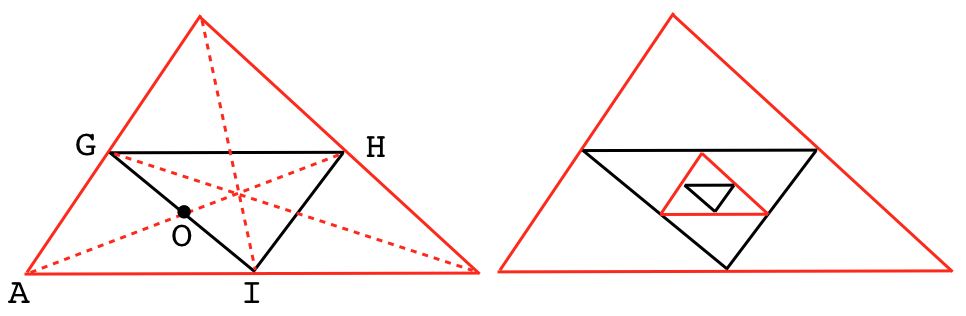
\includegraphics [scale=0.4] {midpoints2.png} \end{center}

Therefore the centroid of $\triangle GHI$ is also the centroid of the parent.  This process can be repeated as many times as we please (right panel).  The triangles get smaller and eventually tend to a point.  That point is on all three midpoint segments.  Therefore, the centroid is a single point.

$\square$

Note:  this is actually a special case of Ceva's theorem, which we proved previously.  But I really like the proof above, which is from Lockhart.

If you know about vectors, it is a good exercise to prove  Ceva's theorem for the centroid using vectors.

\subsection*{algebra of the centroid}

We can locate the centroid by imagining that we find successive midpoints of a length from opposite ends left and right.  

The first point is at $1/2$ of the length (point $O$ on $\triangle GHI$), the second comes back from vertex $H$ by $1/4$ so is at $0.75$ (on the right edge of the small red triangle in the right panel, above).  The third is at $0.5 + 1/8$ (on the left edge of the smallest black triangle).

Every second round we get closer to the centroid  by advancing from the left by
\[ S = \frac{1}{2} +  \frac{1}{8} +  \frac{1}{32}  + \dots \]

Now, we can either assume this sum is finite (for now) or recognize that it is certainly smaller than 
\[ \frac{1}{2} +  \frac{1}{4} +  \frac{1}{8}  + \dots = 1 \]

\begin{center}
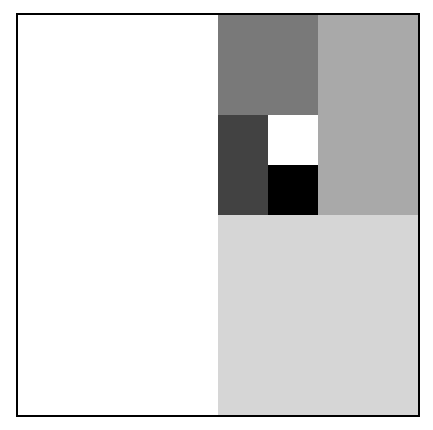
\includegraphics [scale=0.3] {series1.png}
\end{center}

So if
\[ S = \frac{1}{2} +  \frac{1}{8} +  \frac{1}{32}  + \dots \]
then
\[ 2S = 1 +  \frac{1}{4} +  \frac{1}{16}  + \dots \]
and
\[ 3S = 1 +  \frac{1}{2} +  \frac{1}{4} +  \frac{1}{8} + \frac{1}{16}   + \dots \]
\[ = 1 + 1 \]
\[ S = \frac{2}{3} \]

$\square$


\end{document}